\begin{figure*}[t]
	\addtolength{\tabcolsep}{-4.5pt}
	\begin{tabular}{cccccccc}
		& \multicolumn{2}{c}{\toptext{2\resultwidth}{Point estimate}} & \multicolumn{5}{c}{\toptext{5\resultwidth}{Bayesian inference}}\\[-4pt]
		target & loss & optimize & posterior & sample-1 & sample-2 & sample-3& sample-4
		\\
		
\includegraphics[width=\resultwidth]{images/real/bump/out/target.jpg} &
		\includegraphics[width=\resultwidth]{images/real/bump/out/loss.pdf} &
		\includegraphics[width=\resultwidth]{images/real/bump/out/optim.jpg} &
		\includegraphics[width=\resultwidth]{images/real/bump/out/posterior.pdf} &
		\includegraphics[width=\resultwidth]{images/real/bump/out/good1.jpg} &
		\includegraphics[width=\resultwidth]{images/real/bump/out/good2.jpg} &
		\includegraphics[width=\resultwidth]{images/real/bump/out/good3.jpg} &
		\includegraphics[width=\resultwidth]{images/real/bump/out/bad1.jpg}
		\\
		
\includegraphics[width=\resultwidth]{images/real/leather/out/target.jpg} &
		\includegraphics[width=\resultwidth]{images/real/leather/out/loss.pdf} &
		\includegraphics[width=\resultwidth]{images/real/leather/out/optim.jpg} &
		\includegraphics[width=\resultwidth]{images/real/leather/out/posterior.pdf} &
		\includegraphics[width=\resultwidth]{images/real/leather/out/good1.jpg} &
		\includegraphics[width=\resultwidth]{images/real/leather/out/good2.jpg} &
		\includegraphics[width=\resultwidth]{images/real/leather/out/good3.jpg} &
		\includegraphics[width=\resultwidth]{images/real/leather/out/bad1.jpg}
		\\
		
\includegraphics[width=\resultwidth]{images/real/plaster/out/target.jpg} &
		\includegraphics[width=\resultwidth]{images/real/plaster/out/loss.pdf} &
		\includegraphics[width=\resultwidth]{images/real/plaster/out/optim.jpg} &
		\includegraphics[width=\resultwidth]{images/real/plaster/out/posterior.pdf} &
		\includegraphics[width=\resultwidth]{images/real/plaster/out/good1.jpg} &
		\includegraphics[width=\resultwidth]{images/real/plaster/out/good2.jpg} &
		\includegraphics[width=\resultwidth]{images/real/plaster/out/good3.jpg} &
		\includegraphics[width=\resultwidth]{images/real/plaster/out/bad1.jpg}
		\\
%		
\includegraphics[width=\resultwidth]{images/real/flake/out/target.jpg} &
%		\includegraphics[width=\resultwidth]{placeholder/placeholder3.jpg} &
%		\includegraphics[width=\resultwidth]{images/real/flake/out/optim.jpg} &
%		\includegraphics[width=\resultwidth]{placeholder/placeholder3.jpg} &
%		\includegraphics[width=\resultwidth]{images/real/flake/out/good1.jpg} &
%		\includegraphics[width=\resultwidth]{images/real/flake/out/good2.jpg} &
%		\includegraphics[width=\resultwidth]{images/real/flake/out/good3.jpg} &
%		\includegraphics[width=\resultwidth]{placeholder/placeholder3.jpg}
%		\\
%		
\includegraphics[width=\resultwidth]{images/real/metal/out/target.jpg} &
%		\includegraphics[width=\resultwidth]{placeholder/placeholder3.jpg} &
%		\includegraphics[width=\resultwidth]{placeholder/placeholder3.jpg} &
%		\includegraphics[width=\resultwidth]{placeholder/placeholder3.jpg} &
%		\includegraphics[width=\resultwidth]{images/real/metal/out/good1.jpg} &
%		\includegraphics[width=\resultwidth]{images/real/metal/out/good2.jpg} &
%		\includegraphics[width=\resultwidth]{images/real/metal/out/good3.jpg} &
%		\includegraphics[width=\resultwidth]{placeholder/placeholder3.jpg}
%		\\
		
\includegraphics[width=\resultwidth]{images/real/wood/out/target.jpg} &
		\includegraphics[width=\resultwidth]{images/real/wood/out/loss.pdf} &
		\includegraphics[width=\resultwidth]{images/real/wood/out/optim.jpg} &
		\includegraphics[width=\resultwidth]{images/real/wood/out/posterior.pdf} &
		\includegraphics[width=\resultwidth]{images/real/wood/out/good1.jpg} &
		\includegraphics[width=\resultwidth]{images/real/wood/out/good2.jpg} &
		\includegraphics[width=\resultwidth]{images/real/wood/out/good3.jpg} &
		\includegraphics[width=\resultwidth]{images/real/wood/out/bad1.jpg}
		\\
		& & \qquad \qquad \, low &
		\includegraphics[width=\resultwidthpdf]{images/img/colorbar.png} &
		high \qquad \qquad \,& & &
	\end{tabular}
	\caption{\label{fig:real}
		\textbf{Optimization and HMC sampling on real photos.}
		Each row corresponds to a different material. From top: bump, leather, plaster, and wood. Similar to Figure~\protect\ref{fig:synth}, except column 1 here contains real photos, columns 2 and 3 show point estimates (via non-linear optimization), and the remaining columns show HMC sampling results. Please refer to the supplemental material to see more results.
	}
\end{figure*}
